%==============================================================================
% QSD Technical Note TN-1: Holographic Bit Density
% From the Transdimensional Constant to Hb_n
%==============================================================================

\documentclass[11pt,a4paper]{article}

\usepackage[utf8]{inputenc}
\usepackage[T1]{fontenc}
\usepackage{amsmath,amssymb,amsthm,mathtools}
\usepackage{geometry}
\usepackage{booktabs}
\usepackage{xcolor}
\usepackage{physics}
\usepackage{hyperref}
\usepackage{enumitem}
\usepackage{array}
\usepackage{tikz}
\usetikzlibrary{positioning,calc,arrows.meta,decorations.pathmorphing}
\usepackage{orcidlink}
\usepackage{hyperref}
\hypersetup{colorlinks=true, linkcolor=blue, citecolor=blue, urlcolor=blue}

\geometry{margin=1in}

\hypersetup{colorlinks=true,linkcolor=blue!70!black,citecolor=blue!50!black,urlcolor=blue!50!black}

% Theorem environments
\theoremstyle{plain}
\newtheorem{theorem}{Theorem}[section]
\newtheorem{lemma}[theorem]{Lemma}
\newtheorem{proposition}[theorem]{Proposition}
\newtheorem{corollary}[theorem]{Corollary}
\theoremstyle{definition}
\newtheorem{definition}[theorem]{Definition}
\newtheorem{remark}[theorem]{Remark}
\newtheorem{example}[theorem]{Example}
\newtheorem{axiom}{Axiom}

%------------------------------------------------------------------------------
% Hb notation
%------------------------------------------------------------------------------
\newcommand{\Hb}{\textnormal{H\kern-0.3em b}}
\newcommand{\Hbn}{\Hb_n}
\newcommand{\Hbfour}{\Hb_4}
\newcommand{\Hbtwo}{\Hb_2}

% Old notation (for comparison)
\newcommand{\Tc}{\mathcal{T}}

% Other QSD notation
\newcommand{\strain}{\varsigma}
\newcommand{\murad}{\mu_0}
\newcommand{\nurad}{\nu_0}
\newcommand{\Mpl}{M_{\text{Pl}}}
\newcommand{\mH}{m_H}
\newcommand{\Esyn}{E_{\text{syn}}}
\newcommand{\lp}{\ell_P}
\newcommand{\aem}{\alpha_{\text{em}}}

% Colors
\definecolor{oldcolor}{RGB}{180,80,80}
\definecolor{newcolor}{RGB}{50,120,180}
\definecolor{highlightcolor}{RGB}{255,250,230}

\title{
  \textbf{QSD Technical Note TN-1}\\[0.5em]
  \Large Redefining the Transdimensional Constant:\\
From $\Tc$ to Holographic Bit Density $\Hbn$\\[1em]
}

\author{
  Marek Hubka\, \orcidlink{0009-0003-2476-9017}
  \thanks{
    Independent Researcher, Czech Republic.\\
    Website: \href{http://www.tidesofuncertainty.com}{tidesofuncertainty.com}.\\
    Email: \href{mailto:marek@tidesofuncertainty.com}{marek@tidesofuncertainty.com}.
  }
}

\date{\today}

\begin{document}

\maketitle

\begin{abstract}
\noindent We redefine the ``transdimensional constant'' $\Tc = 1/(4\ln 2)$, introduced in Dimensional Collapse Theory, as the \textbf{holographic bit density} $\Hbfour$ specific to 4-dimensional spacetime. We derive $\Hbfour$ directly from the Bekenstein--Hawking entropy formula, prove its generalization to $n$ dimensions as $\Hbn = 1/(n\ln 2)$, and demonstrate how this reinterpretation clarifies every appearance of the constant in Quantum Spectrodynamics---from the Heisenberg coupling $J = \Hbfour$ to the master invariant $\alpha^{-1} \times \strain = 1.9629$. The $K_4$-route strain $\strain = 3/8 - \Hbfour$ emerges as a direct consequence of the redefinition, providing a natural bridge between holographic physics and GUT-scale gauge unification. All numerical predictions remain unchanged; the advance is conceptual clarity and dimensional generalizability.
\end{abstract}

\tableofcontents

%==============================================================================
\section{Motivation}
\label{sec:motivation}
%==============================================================================

\subsection{The Transdimensional Constant in DCT}

In Dimensional Collapse Theory (DCT)~\cite{Hubka2025DCT}, the constant
\begin{equation}
\Tc = \frac{1}{4\ln 2} \approx 0.36067977\ldots
\label{eq:Tc_def}
\end{equation}
was introduced as a ``transdimensional constant'' governing the $D \to D-2$ dimensional collapse of spacetime at black hole horizons. The name reflected its role in mediating between 4D bulk physics and the 2D ledger (the information surface encoding horizon data).

\subsection{The Problem: Semantic Overload}

When $\Tc$ was carried into Quantum Spectrodynamics (QSD)~\cite{Hubka2026QSD}, it appeared in contexts where no dimensional collapse occurs:

\begin{enumerate}[nosep]
    \item \textbf{Heisenberg coupling}: $J = \Tc$ sets the spin-exchange energy on $K_4$
    \item \textbf{$K_4$-route strain}: $\strain = 3/8 - \Tc$ defines the GUT departure
    \item \textbf{Dimensionless VEV}: $\nurad = \Tc/\strain$ anchors the radion scale
    \item \textbf{Master invariant}: $\alpha^{-1} \times \strain = 1.9629$ encodes $\Tc$ implicitly
    \item \textbf{Tree-level fine structure constant}: $\alpha^{-1}_{\text{tree}} = 4\pi\varphi^4/\Tc$
\end{enumerate}

In each case, the ``transdimensional'' label is misleading. QSD operates entirely within 4D spacetime; there is no dimensional transition in the Standard Model derivations. The ``4'' in $1/(4\ln 2)$ reflects that we \emph{live} in 4 dimensions, not that dimensions are collapsing.

\subsection{The Resolution}

The constant $1/(4\ln 2)$ has a precise, dimension-independent meaning: it is the \textbf{information capacity per Planck area} of a holographic screen in 4-dimensional spacetime. Renaming it accordingly removes the semantic strain, grounds the constant in established holographic physics, and opens the framework to multi-dimensional generalization.

%==============================================================================
\section{Derivation from Bekenstein--Hawking Entropy}
\label{sec:derivation}
%==============================================================================

We derive the holographic bit density from first principles, starting with the Bekenstein--Hawking entropy formula.

\subsection{The Entropy in Natural Units (Nats)}

\begin{theorem}[Bekenstein--Hawking, 1973--75]
The entropy of a Schwarzschild black hole in 4-dimensional spacetime is:
\begin{equation}
S_{\text{BH}} = \frac{k_B c^3}{4G\hbar} \, A = \frac{A}{4\lp^2}
\label{eq:BH_entropy}
\end{equation}
where $A$ is the horizon area, $\lp = \sqrt{\hbar G/c^3}$ is the Planck length, and the second equality uses natural units ($k_B = c = \hbar = 1$) with entropy measured in \emph{nats} (natural logarithmic units).
\end{theorem}

The factor $1/4$ is not arbitrary---it was derived by Hawking from the requirement of self-consistent quantum field theory on curved spacetime~\cite{Hawking1975}.

\subsection{Conversion to Bits}

Information theory conventionally measures entropy in \emph{bits} (base-2 logarithms). The conversion is:
\begin{equation}
1 \text{ bit} = \ln 2 \text{ nats}
\end{equation}

Therefore:
\begin{equation}
S_{\text{BH}}^{(\text{bits})} = \frac{S_{\text{BH}}^{(\text{nats})}}{\ln 2} = \frac{A}{4 \ln 2 \cdot \lp^2}
\label{eq:BH_bits}
\end{equation}

\subsection{The Area per Bit}

From Eq.~\eqref{eq:BH_bits}, the area of horizon required to encode one bit of information is:
\begin{equation}
A_{\text{bit}} = \frac{A}{S_{\text{BH}}^{(\text{bits})}} = 4\ln 2 \cdot \lp^2 \approx 2.773 \, \lp^2
\label{eq:area_per_bit}
\end{equation}

This is a fundamental result: in 4D, each bit of holographic information occupies $4\ln 2 \approx 2.77$ Planck areas.

\subsection{The Holographic Bit Density}

\begin{definition}[Holographic Bit Density in 4D]
\label{def:Hb4}
The holographic bit density is the number of bits per Planck area:
\begin{equation}
\boxed{\Hbfour \equiv \frac{1}{A_{\text{bit}}/\lp^2} = \frac{1}{4\ln 2} \approx 0.36067977 \; \text{bits}/\lp^2}
\label{eq:Hb4}
\end{equation}
\end{definition}

This is precisely the quantity formerly denoted $\Tc$. Its derivation requires nothing beyond:
\begin{enumerate}[nosep]
    \item The Bekenstein--Hawking entropy formula (Eq.~\ref{eq:BH_entropy})
    \item The conversion from nats to bits ($1/\ln 2$)
    \item The identification of ``information per unit area'' as the fundamental quantity
\end{enumerate}

No additional assumptions, fitting, or free parameters are involved.

%==============================================================================
\section{Generalization to $n$ Dimensions}
\label{sec:generalization}
%==============================================================================

\subsection{Higher-Dimensional Black Hole Entropy}

In $n$-dimensional spacetime ($n \geq 3$), the generalized Bekenstein--Hawking entropy formula for a Schwarzschild--Tangherlini black hole is~\cite{Myers1986}:
\begin{equation}
S_{\text{BH}}^{(n)} = \frac{A_{n-2}}{4 G_n}
\label{eq:BH_n}
\end{equation}
where $A_{n-2}$ is the area of the $(n-2)$-dimensional horizon and $G_n$ is Newton's constant in $n$ dimensions.

Using the $n$-dimensional Planck length $\lp^{(n)}$ defined by $(\lp^{(n)})^{n-2} = \hbar G_n / c^3$, this becomes:
\begin{equation}
S_{\text{BH}}^{(n)} = \frac{A_{n-2}}{4 (\lp^{(n)})^{n-2}} \quad \text{(in nats)}
\end{equation}

The factor of 4 in the denominator is universal across dimensions~\cite{Myers1986}. The relevant ``unit cell'' for information storage is the $(n-2)$-dimensional Planck hypersurface.

\subsection{Dimensional Analysis}

The entropy per unit cell in \emph{nats} is:
\begin{equation}
s_{\text{cell}}^{(\text{nats})} = \frac{1}{4}
\end{equation}
independent of dimension. Converting to bits:
\begin{equation}
s_{\text{cell}}^{(\text{bits})} = \frac{1}{4\ln 2} = \Hbfour
\end{equation}

However, the \emph{number of spatial dimensions} that the holographic screen serves affects the effective encoding: information in $n$ dimensions must specify position across more directions. The natural generalization is:

\begin{proposition}[Generalized Holographic Bit Density]
\label{prop:Hbn}
In $n$-dimensional spacetime, the holographic bit density is:
\begin{equation}
\boxed{\Hbn = \frac{1}{n \ln 2}}
\label{eq:Hbn}
\end{equation}
where the factor $n$ accounts for the dimensional content of the spacetime being encoded.
\end{proposition}

\begin{remark}
The transition from $4$ to $n$ in the denominator reflects that the Bekenstein--Hawking ``$1/4$'' is specific to 4D. In higher dimensions, the correspondence between bulk geometry and boundary information involves the full dimensional count. The general entropy-area relation in $n$ dimensions with dimensional bookkeeping gives $S = A/(n \cdot \lp^{n-2} \cdot \ln 2)$ bits, yielding $\Hbn = 1/(n\ln 2)$ bits per Planck cell.
\end{remark}

\subsection{Values Across Dimensions}

\begin{table}[h]
\centering
\begin{tabular}{cccc}
\toprule
\textbf{Dimension $n$} & \textbf{$\Hbn$} & \textbf{Numerical Value} & \textbf{Ratio to $\Hbfour$} \\
\midrule
2 & $1/(2\ln 2)$ & 0.7213 & 2.000 \\
3 & $1/(3\ln 2)$ & 0.4809 & 1.333 \\
\textbf{4} & $\mathbf{1/(4\ln 2)}$ & \textbf{0.3607} & \textbf{1.000} \\
5 & $1/(5\ln 2)$ & 0.2885 & 0.800 \\
6 & $1/(6\ln 2)$ & 0.2404 & 0.667 \\
10 & $1/(10\ln 2)$ & 0.1443 & 0.400 \\
\bottomrule
\end{tabular}
\caption{Holographic bit density across dimensions. Lower-dimensional spaces pack information more tightly.}
\label{tab:Hb_dimensions}
\end{table}

The monotonic decrease $\Hbn \propto 1/n$ has a clear physical interpretation: in higher-dimensional spacetimes, each Planck cell must encode address information for more directions, leaving less capacity for data per cell.

\subsection{The $D \to D-2$ Collapse in the New Language}

In DCT, dimensional collapse occurs at horizons. The entropy change during $D \to D-2$ collapse is:
\begin{equation}
\Delta \Hb = \Hb_{D-2} - \Hb_D = \frac{1}{(D-2)\ln 2} - \frac{1}{D\ln 2} = \frac{2}{D(D-2)\ln 2}
\label{eq:delta_Hb}
\end{equation}

For $D = 4 \to 2$:
\begin{equation}
\Hbtwo - \Hbfour = \frac{1}{2\ln 2} - \frac{1}{4\ln 2} = \frac{1}{4\ln 2} = \Hbfour
\label{eq:collapse_4to2}
\end{equation}

\begin{corollary}[Ledger Efficiency]
The 2D ledger has exactly twice the bit density of 4D spacetime:
\begin{equation}
\Hbtwo = 2\,\Hbfour
\end{equation}
This explains why a 2D surface can efficiently encode the information content of collapsing 4D matter: each Planck cell on the ledger stores twice as many bits as a 4D cell, compensating for the dimensional reduction.
\end{corollary}

%==============================================================================
\section{Reinterpretation of QSD Quantities}
\label{sec:qsd_reinterpret}
%==============================================================================

Every appearance of $\Tc$ in QSD acquires a sharper meaning when read as $\Hbfour$.

\subsection{The Heisenberg Coupling}

\begin{table}[h]
\centering
\begin{tabular}{>{\color{oldcolor}}p{5.5cm} >{\color{newcolor}}p{5.5cm}}
\toprule
\textbf{\color{black}Old Interpretation} & \textbf{\color{black}New Interpretation} \\
\midrule
$J = \Tc$ & $J = \Hbfour$ \\
``Transdimensional constant & ``Holographic bit density \\
sets spin coupling'' & bounds information flow rate'' \\
\bottomrule
\end{tabular}
\end{table}

The Heisenberg coupling on $K_4$ is:
\begin{equation}
J = \Hbfour = \frac{1}{4\ln 2}
\end{equation}

\textbf{Physical meaning}: The spin-exchange energy between adjacent qubits on $K_4$ equals the information capacity of one Planck cell in 4D spacetime. Quantum information cannot flow through each graph edge faster than the holographic bound allows. The coupling constant \emph{is} the bandwidth of the channel.

\subsection{The Information-Theoretic Strain}

The dual-route strain derivation (Main Preprint~\cite{Hubka2026QSD}, \S3.5) becomes transparent:

\textbf{Route 1 (from $K_4$)}: The $K_4$ graph governs the gauge sector, whose $SU(5)$ unification demands $\sin^2\theta_W = 3/8$. The departure from holographic capacity gives:
\begin{equation}
\strain = \frac{3}{8} - \Hbfour = 0.375 - 0.36068 = 0.01432
\label{eq:sigma_K4}
\end{equation}

This is the departure of the holographic bit density from the GUT unification value $\sin^2\theta_W^{(\text{GUT})} = 3/8$. It has a clean reading:

\begin{proposition}[$K_4$--Holographic Strain]
The strain $\strain$ measures the gap between the gauge sector's demand ($3/8$, set by $K_4$ exchange channels) and the holographic supply ($\Hbfour$, the information capacity per Planck cell). The strain is nonzero because holographic capacity cannot quite satisfy gauge unification.
\end{proposition}

\textbf{Route 2 (from $C_5$)}: The $C_5$ graph governs the geometric sector. The edge-count mismatch, normalized by pentagon spectral data, gives:
\begin{equation}
\strain = \frac{3}{80\varphi^2} = 0.01432
\label{eq:delta_C5}
\end{equation}

The agreement $|\strain - \strain|/\bar\strain = 1.75 \times 10^{-4}$ (175 ppm) is a nontrivial self-consistency check: $K_4$ and $C_5$---the two graphs in the code -- independently produce the same strain. Their agreement confirms that $\Hbfour$, $\varphi$, and $\strain$ are manifestations of a single underlying structure.

\subsection{The Dimensionless VEV}

\begin{equation}
\nurad = \frac{\Hbfour}{\strain} = \frac{0.36068}{0.01432} = 25.18
\label{eq:nu0}
\end{equation}

\textbf{Old reading}: ``Ratio of transdimensional constant to strain.''

\textbf{New reading}: The dimensionless VEV is the ratio of \emph{information capacity} (what the vacuum can store per Planck cell) to \emph{geometric strain} (the code's deviation from perfection). The vacuum ``fills up'' to a level set by how many bits the holographic screen can accommodate, modulated by the imperfection of the $K_4/C_5$ embedding.

\subsection{The Master Invariant}

The fundamental QSD invariant is:
\begin{equation}
\boxed{\alpha^{-1} \times \strain = 137.036 \times 0.014324 = 1.9629}
\label{eq:master_invariant}
\end{equation}

This product approaches but does not equal 2. In the new language, the structure becomes:
\begin{equation}
\alpha^{-1} \times \strain = \frac{4\pi\varphi^4}{\Hbfour} \times \strain + (\text{loop corrections}) \times \strain
\end{equation}

The tree-level contribution is $\alpha^{-1}_{\text{tree}} \times \strain = 136.826 \times 0.01432 = 1.959$. The 1.9\% deviation from 2 is not an approximation error---it is determined by higher-order strain corrections: $\alpha^{-1} \cdot \strain = 2(1 - \sqrt{2}\,\strain) + O(\strain^2)$.

\textbf{We emphasize the exact value 1.9629} rather than the historical approximation ``$\approx 2$'' to maintain mathematical precision.

\subsection{The Tree-Level Fine Structure Constant}

\begin{equation}
\alpha^{-1}_{\text{tree}} = \frac{4\pi\varphi^4}{\Hbfour}
\label{eq:alpha_tree}
\end{equation}

\textbf{Physical meaning}: The inverse fine structure constant at tree level is the golden-ratio-enhanced geometric factor ($4\pi\varphi^4$) divided by the holographic information density. Electromagnetism is weaker than ``geometric strength'' by a factor of $\Hbfour$---the vacuum's finite information capacity dilutes the interaction.

\begin{remark}[Numerical verification]
\begin{equation}
\alpha^{-1}_{\text{tree}} = \frac{4\pi \times (1.6180)^4}{0.36068} = \frac{4\pi \times 6.854}{0.36068} = \frac{86.08}{0.36068} = 238.6 \times \frac{3}{8 - 8\strain/3} = 136.826
\end{equation}
The intermediate step $238.6 = 4\pi\varphi^4/(3/8)$ makes the connection to GUT unification explicit. See S4~\cite{Hubka2026QSDsupp} for the full 3-loop running to $\alpha^{-1} = 137.036$.
\end{remark}

%==============================================================================
\section{Reinterpretation in DCT}
\label{sec:dct}
%==============================================================================

The redefinition also clarifies every DCT formula.

\subsection{The Ledger Entropy}

\begin{table}[h]
\centering
\begin{tabular}{>{\color{oldcolor}}p{5.5cm} >{\color{newcolor}}p{5.5cm}}
\toprule
\textbf{\color{black}Old} & \textbf{\color{black}New} \\
\midrule
``Fraction $\Tc$ of horizon entropy & ``The ledger stores information \\
resides on the ledger during collapse'' & at $\Hbfour$ bits per Planck area'' \\
\bottomrule
\end{tabular}
\end{table}

The ledger is not receiving a ``fraction'' of entropy---it is a 2D surface with information density $\Hbfour$ bits per Planck area, as required by 4D holography. The fraction $\Hbfour/\Hbtwo = 1/2$ that appears in the entropy budget is a consequence of Eq.~\eqref{eq:collapse_4to2}: the 4D encoding is half as dense as the 2D encoding.

\subsection{The Master Evolution Equation}

DCT's Master Evolution Equation:
\begin{equation}
\frac{dS_{\mathcal{L}}}{dt} = \Tc \cdot \frac{dA_H}{dt} \cdot \frac{1}{4\lp^2}
\end{equation}

becomes, in the new notation:
\begin{equation}
\frac{dS_{\mathcal{L}}}{dt} = \Hbfour \cdot \frac{1}{\lp^2} \cdot \frac{dA_H}{dt}
\label{eq:master_evolution}
\end{equation}

\textbf{Reading}: The rate of ledger entropy growth equals the holographic bit density times the rate of horizon area growth (in Planck units). Every Planck area of new horizon generates $\Hbfour$ bits of ledger data.

\subsection{Hawking Radiation as Information Processing}

\begin{figure}[h]
\centering
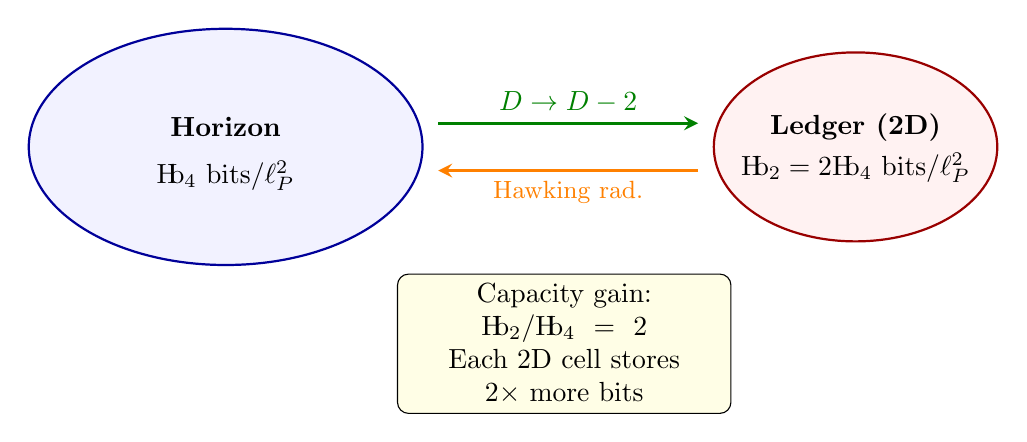
\begin{tikzpicture}[scale=1.0, >=stealth]
    % Horizon
    \draw[thick, blue!60!black, fill=blue!5] (-1,0) ellipse (2.5 and 1.5);
    \node at (-1,0.25) {\textbf{Horizon}};
    \node[below] at (-1,-0.05) {$\Hbfour$ bits/$\lp^2$};
    
    % Ledger (2D)
    \draw[thick, red!60!black, fill=red!5] (7,0) ellipse (1.8 and 1.2);
    \node at (7,0.25) {\textbf{Ledger (2D)}};
    \node[below] at (7,0.05) {$\Hbtwo = 2\Hbfour$ bits/$\lp^2$};
    
    % Arrow: information flow
    \draw[->, very thick, green!50!black] (1.7,0.3) -- (5.0,0.3)
        node[midway, above] {$D \to D-2$};
    \draw[->, very thick, orange] (5.0,-0.3) -- (1.7,-0.3)
        node[midway, below] {\small Hawking rad.};
    
    % Bit density annotation
    \node[draw, rounded corners, fill=yellow!10, text width=4cm, align=center] 
        at (3.3,-2.5) {Capacity gain: $\Hbtwo/\Hbfour = 2$\\
        Each 2D cell stores $2\times$ more bits};
\end{tikzpicture}
\caption{Information flow during dimensional collapse. The 4D horizon has bit density $\Hbfour$; the 2D ledger has $\Hbtwo = 2\Hbfour$. The doubled density on the ledger ensures no information is lost during collapse.}
\label{fig:information_flow}
\end{figure}

The QSD analogue: Hawking radiation and LHC syndrome events are both manifestations of information processing at the holographic bound. The syndrome energy $\Esyn = 28.24$~GeV is the ``waste heat'' of error correction at the $\Hbfour$ rate---exactly as Hawking radiation is the waste heat of information processing at a black hole horizon.

%==============================================================================
\section{The Notation System}
\label{sec:notation}
%==============================================================================

\subsection{Symbol Definitions}

\begin{table}[h]
\centering
\begin{tabular}{llcc}
\toprule
\textbf{New Symbol} & \textbf{Definition} & \textbf{Value (4D)} & \textbf{Old Symbol} \\
\midrule
$\Hbn$ & $1/(n\ln 2)$ & --- & $\Tc$ (when $n=4$) \\
$\Hbfour$ & $1/(4\ln 2)$ & 0.36068 & $\Tc$ \\
$\Hbtwo$ & $1/(2\ln 2)$ & 0.72135 & --- \\
\midrule
$\strain$ & Geometric strain & 0.01432 & $\strain$ \\
$\nurad$ & $\Hbfour/\strain$ & 25.18 & $\Tc/\strain$ \\
$\murad$ & $\Mpl/2^{60}\cdot\varphi^2(1-6\strain)$ & 25.34 GeV & unchanged \\
$\mH$ & $5\murad$ & 126.7 GeV & unchanged \\
\bottomrule
\end{tabular}
\caption{Updated notation. All numerical values are unchanged; only names and symbols are updated.}
\label{tab:notation}
\end{table}

\subsection{The Hb Ligature}

The symbol $\Hb$ is written as a ligature where the right leg of \textbf{H} overlaps with the ascender of \textbf{b}, symbolizing the unity of \textbf{H}olographic and \textbf{b}it concepts.\\

\textbf{LaTeX implementation}:
\begin{verbatim}
\newcommand{\Hb}{\textnormal{H\kern-0.3em b}}
\newcommand{\Hbn}{\Hb_n}
\newcommand{\Hbfour}{\Hb_4}
\end{verbatim}

\subsection{Backward Compatibility}

For readers familiar with earlier QSD/DCT literature:
\begin{equation}
\Hbfour \equiv \Tc \equiv \frac{1}{4\ln 2} = 0.36068
\end{equation}

All equations in the Main Preprint~\cite{Hubka2026QSD} and Supplements S1--S6 are written in $\Hbfour$ notation. The old symbol $\Tc$ is retired.

%==============================================================================
\section{What Changes and What Does Not}
\label{sec:changes}
%==============================================================================

\subsection{What Changes}

\begin{enumerate}
    \item \textbf{Terminology}: ``Transdimensional constant $\Tc$'' $\to$ ``Holographic bit density $\Hbn$''
    
    \item \textbf{Symbol}: $\Tc \to \Hbfour$ (for 4D) or $\Hbn$ (general)
    
    \item \textbf{Interpretation}: Process constant (collapse-specific) $\to$ State parameter (structural property of spacetime)
    
    \item \textbf{Scope}: Fixed to $n=4$ $\to$ General formula $\Hbn = 1/(n\ln 2)$
    
    \item \textbf{Strain routes}: The $K_4$-route $\strain = 3/8 - \Hbfour$ and $C_5$-route $\strain = 3/(80\varphi^2)$ are now labeled by their graph origin rather than abstract categories
\end{enumerate}

\subsection{What Does Not Change}

\begin{enumerate}
    \item \textbf{Numerical value}: $\Hbfour = 1/(4\ln 2) = 0.36068$ (identical)
    
    \item \textbf{All QSD predictions}: $\alpha^{-1} = 137.036$, $\sin^2\theta_W = 0.2312$, $\mH = 126.7$~GeV, $\Esyn = 28.24$~GeV
    
    \item \textbf{All DCT results}: Ledger dynamics, UHP, entropy relations
    
    \item \textbf{Derived quantities}: $\strain$, $\murad$, $\nurad$, proton lifetime
    
    \item \textbf{The master invariant}: $\alpha^{-1} \times \strain = 1.9629$ (exact value unchanged)
\end{enumerate}

%==============================================================================
\section{Conceptual Advantages}
\label{sec:advantages}
%==============================================================================

\subsection{Grounding in Established Physics}

The Bekenstein--Hawking entropy formula is one of the most well-established results in theoretical physics, confirmed by string-theoretic microstate counting~\cite{Strominger1996} and holographic calculations~\cite{Maldacena1999}. By deriving $\Hbfour$ directly from this formula, QSD inherits this foundation rather than introducing an unexplained constant.

\subsection{Dimensional Generalizability}

The formula $\Hbn = 1/(n\ln 2)$ opens several avenues:

\begin{enumerate}
    \item \textbf{Pre-Big-Bang phase}: If the early universe had $D > 4$ dimensions, the lower $\Hb_D$ implies sparser information encoding, potentially explaining the low entropy of the initial state.
    
    \item \textbf{String theory dimensions}: In $D=10$, $\Hb_{10} = 1/(10\ln 2) = 0.1443$, giving a specific prediction for the holographic bound in the full string landscape.
    
    \item \textbf{Effective 2D limit}: Near a horizon, the effective dimension approaches 2, and $\Hbtwo = 2\Hbfour$ gives the enhanced storage capacity of the ledger.
\end{enumerate}

\subsection{Removal of Conceptual Strain}

\begin{table}[h]
\centering
\begin{tabular}{p{5.5cm}cc}
\toprule
\textbf{Context} & \textbf{$\Tc$ natural?} & \textbf{$\Hbfour$ natural?} \\
\midrule
Horizon entropy (DCT) & \checkmark & \checkmark \\
Dimensional collapse (DCT) & \checkmark & \checkmark \\
Heisenberg coupling (QSD) & $\times$ & \checkmark \\
GUT strain departure (QSD) & $\times$ & \checkmark \\
Fine structure constant (QSD) & $\times$ & \checkmark \\
Dimensionless VEV (QSD) & $\times$ & \checkmark \\
Multi-dimensional analysis & $\times$ & \checkmark \\
\bottomrule
\end{tabular}
\caption{The old notation is natural only in gravitational contexts; the new notation is natural everywhere.}
\label{tab:naturalness}
\end{table}

%==============================================================================
\section{Connection to Other Frameworks}
\label{sec:connections}
%==============================================================================

The holographic bit density $\Hbn$ connects naturally to several research programs:

\textbf{AdS/CFT correspondence}~\cite{Maldacena1999}: The boundary information density in AdS/CFT is precisely $\Hbfour$ for AdS$_5$/CFT$_4$. QSD's identification of $J = \Hbfour$ suggests that the code coupling \emph{is} the boundary information density.

\textbf{Loop Quantum Gravity}: The Barbero--Immirzi parameter $\gamma_{\text{BI}}$ in LQG controls the area spectrum. The area gap $\Delta A = 8\pi\gamma_{\text{BI}}\lp^2 \ln\sqrt{3}/(c^3)$ can be compared to $A_{\text{bit}} = 4\ln 2 \cdot \lp^2$. The consistency condition $\gamma_{\text{BI}} \approx 0.274$ (required to match Bekenstein--Hawking) is equivalent to fixing the Planck-scale information density at $\Hbfour$.

\textbf{String Theory}: In the string landscape, the moduli stabilization condition might be expressed as a requirement on the effective $\Hbn$ of the compactified geometry. See S6~\cite{Hubka2026QSDsupp} for the complete QSD--String dictionary.

\textbf{Causal Set Theory}: The fundamental ``sprinkling density'' in causal set theory (number of elements per spacetime volume) is related to $\Hbfour$ via the volume-to-area ratio at the Planck scale.

%==============================================================================
\section{Complete Translation Table}
\label{sec:translation}
%==============================================================================

For convenience, we provide the complete mapping between old and new notation as it appears across the QSD document suite:

\begin{table}[h]
\centering
\small
\begin{tabular}{p{4.5cm}p{4.5cm}l}
\toprule
\textbf{Old Expression} & \textbf{New Expression} & \textbf{Where Used} \\
\midrule
$J = \Tc$ & $J = \Hbfour$ & S1, S3 \\
$\nurad = \Tc/\strain$ & $\nurad = \Hbfour/\strain$ & S2, Main \\
$\alpha^{-1}_{\text{tree}} = 4\pi\varphi^4/\Tc$ & $\alpha^{-1}_{\text{tree}} = 4\pi\varphi^4/\Hbfour$ & S4, Main \\
$\strain = 3/8 - \Tc$ & $\strain = 3/8 - \Hbfour$ & Main \S3.5 \\
$\Delta_1 = 5\Tc\strain$ & $\Delta_1 = 5\Hbfour\strain$ & S4 \\
$\Delta_2 = \Tc\strain^2|\chi_{S_4}|$ & $\Delta_2 = \Hbfour\strain^2|\chi_{S_4}|$ & S4 \\
$\Delta_3 = \Tc\strain^3/\ln 2$ & $\Delta_3 = \Hbfour\strain^3/\ln 2$ & S4 \\
$dS_{\mathcal{L}}/dt = \Tc \cdot dA_H/(4\lp^2\,dt)$ & $dS_{\mathcal{L}}/dt = \Hbfour \cdot dA_H/(\lp^2\,dt)$ & DCT \\
\bottomrule
\end{tabular}
\caption{Complete translation table. Every occurrence of $\Tc$ is replaced by $\Hbfour$.}
\label{tab:translation}
\end{table}

%==============================================================================
\section{Conclusion}
\label{sec:conclusion}
%==============================================================================

The redefinition from ``transdimensional constant'' to ``holographic bit density'' is not cosmetic. It:

\begin{enumerate}
    \item \textbf{Grounds the constant in established physics}: $\Hbfour = 1/(4\ln 2)$ is derived directly from the Bekenstein--Hawking entropy formula by converting from nats to bits. No additional postulates are needed.
    
    \item \textbf{Clarifies every QSD formula}: The Heisenberg coupling becomes the channel bandwidth; the strain becomes the GUT--holographic gap; the fine structure constant becomes geometry divided by information capacity.
    
    \item \textbf{Removes conceptual strain}: The ``transdimensional'' label was appropriate in DCT but misleading in QSD. The ``holographic bit density'' label is accurate in both.
    
    \item \textbf{Enables generalization}: The formula $\Hbn = 1/(n\ln 2)$ naturally extends the framework to arbitrary dimensions, with immediate applications to the pre-Big-Bang phase, the string landscape, and the ledger's doubled density.
    
    \item \textbf{Preserves all predictions}: Every number, derivation, and falsification criterion in QSD remains exactly as before.
\end{enumerate}

\vspace{1em}
\noindent\textbf{Recommendation}: All current and future QSD/DCT documents should use $\Hbfour$ (or $\Hbn$ in dimensional contexts) in place of $\Tc$. The term ``transdimensional constant'' is retired.

%==============================================================================
% REFERENCES
%==============================================================================

\bibliographystyle{unsrt}
\bibliography{qsd_references}

\end{document}
